\documentclass[a4paper,12pt,russian]{article}

\usepackage{geometry}
\geometry{a4paper,top=2cm,bottom=2cm,left=2cm,right=2cm} %% отступы и т.п.

%% чтоб работал русский язык
\usepackage[utf8]{inputenc}
\usepackage[russian]{babel}

%% для математических символов
\usepackage{amsmath, amsthm, amssymb}

%% листинги кода
\usepackage{listings}
\usepackage{courier}
\lstset{
  language=c++,
  basicstyle=\footnotesize\sffamily,
  keywordstyle=\bfseries,
  stringstyle=\ttfamily,
  numberstyle=\tiny,
  numbers=left
}

%% картинки
\usepackage[pdftex]{graphicx}
\usepackage[small, bf, labelsep=period]{caption}
\graphicspath{{img/}}
\usepackage{multicol}

%% листинги программ
\usepackage{moreverb}
\usepackage[noend]{algorithmic}
\algsetup{indent=2em, linenosize=\small, linenodelimiter=}

%% чтоб первый абзац был с отступом
\usepackage{indentfirst}

%% всякое для удобства разметки
%\newcommand{\remark}[1]{~~\textit{\textbf{(#1)}}}
\newcommand{\remark}[1]{\footnote{#1}}

\newcommand{\picref}[1]{\textbf{рис.~\ref{#1}}}

\newtheorem*{definition}{Определение}

\begin{document}
\begin{titlepage}
	\begin{center}
		\Large
		Московский~государственный~университет\\
		имени М.В.~Ломоносова\\[0.5em]
		\large
		Факультет~вычислительной~математики~и~кибернетики\\
		Кафедра~системного~программирования
	\end{center}

\vskip 14em
	\begin{center}
		\LARGE
		Введение в дипломную работу\\
		\textbf{``Восстановление определений классов в программах на языке Си++ средствами динамического анализа''}\\
	\end{center}
\vskip 6em
	\begin{flushright}
		\large
		Выполнил~студент 527~группы\\
		Прохоренков~П.В.\\
		\vspace{2cm}
		Научный руководитель\\
		к.ф-м.н, доц. Чернов~А.В.\\
\end{flushright}
\vfill
	\begin{center}
		\Large
		Москва\\
		2009
	\end{center}
\end{titlepage}

\tableofcontents

\newpage

\addcontentsline{toc}{section}{Введение}
\section*{Введение}
\emph{Трансформация программы} --- это процесс перевода одной программы в другую с сохранением семантики.
Этот термин также используется для самого алгоритма, осуществляющего такой перевод.
Языки, на которых написаны трансформируемая программа и получающаяся программа, называются \emph{исходным} и \emph{целевым} языками, соответственно.

\emph{Обратная инженерия} является процессом анализа системы, имеющим 2 цели: восстановление компонент системы и их взаимных связей, и создание описания системы в другой форме с более высоким уровнем абстракции

\emph{Декомпиляция} представляет собой частный случай обратной инженерии, это трансформация программы, которая восстанавливает код на языке высокого уровня по исполняемому файлу программы.
Декомпиляция является обратным преобразованием к компиляции.
Методы декомпиляции использовались, начиная с 60-х годов для облегчения переноса программ с одной платформы на другую.
Далее, декомпиляция применялась для восстановления утраченного исходного кода, отладки программ, обнаружения вирусов, восстановления алгоритмов работы программ.

Декомпиляция имеет множество применений:
\begin{itemize}
\item{\textbf{Поиск ошибок}}
\item{\textbf{Поиск уязвимостей}}
\item{\textbf{Поиск вредоносного кода}}
\item{\textbf{Верификация}}
\item{\textbf{Восстановление алгоритма работы}}
\item{\textbf{Создание совместимых программ}}
\item{\textbf{Оптимизация}} Например, старая программа, скомпилированная для старого процессора, может быть перекомпилирована под новый с использованием всех существующих оптимизаций.
\item{\textbf{Портирование на другую платформу}}
\item{\textbf{Восстановление утраченного исходного кода}}
\item{\textbf{Восстановление протоколов обмена программ, исходные коды которых утрачены}}
\end{itemize}

В данной работе будет рассматриваться декомпиляция программ, изначально написанных на языке Си++.
Язык Си++ является языком общего назначения с поддержкой объектно-ориентированной парадигмы программирования \cite{strstr}ю Этот язык получил широкое распространение, и существует множество программ, написанных на нем.

Одной из подзадач декомпиляции является восстановление типов данных высокого уровня, как базовых, так и производных.
В программах на языках высокого уровня разработчику ПО доступно множество различных типов данных.
В их число входят и составные типы данных, во многих случаях размещаемые в динамической памяти.

Ассемблер --- бестиповый язык, следовательно утрачивается информация о высокоуровневых типах данных, которая могла бы помочь аналитику понять анализируемую программу.
Базовые типы после компиляции становятся трудно различимыми, например, на многих 32-разрядных архитектурах \texttt{int}, \texttt{unsigned int} и \texttt{void *} будут храниться в одних и тех-же регистрах размером 4 байта и обрабатываться одним множеством команд.

Помимо базовых типов требуется восстанавливать производные типы данных, такие как классы и их иерархию.
Использование статических методов анализа для решения этой задачи осложняется
тем, что необходимо проведение анализа потоков данных и управления, точное восстановление которых статическими методами невозможно.

Динамический анализ во многих случаях позволяет получать недостающую информацию. Но к числу его недостатков надо отнести необходимость запуска исследуемой программы.
Это требует получения входных данных, в обработке которых будут задействованы все интересующих исследователя участки кода.
Также, в некоторых случаях необходимы большие вычислительные ресурсы из-за накладных расходов инструментария анализа.

Знание иерархии классов, используемых в анализируемой программе может иметь большое значение для специалиста. Например, многие алгоритмы могут быть распознаны по используемым в них структурам данных.

Данная работа посвящена восстановлению иерархий классов по бинарному коду в программах, написанных на языке Си++.
Восстановление проходит при помощи динамического анализа программы.

\newpage
\section{Постановка задачи}
В декомпиляторе \texttt{TyDec} \cite{tydec}, разрабатываемом в ИСП РАН, реализовано статическое восстановление производных типов данных \cite{typereconstruction}.
Требуется разработать и реализовать инструментальное средство, использующее методы динамического анализа для восстановления иерархии классов, используемых в анализируемой программе.
Результатом работы средства должно являться наиболее полно восстановленное:
\begin{enumerate}
\item Множество классов.
\item Частичное отношение наследования между классами.
\item Таблица виртуальных функций для каждого из классов.
\item Список полей для каждого из классов.
\item Частичное отношение ассоциации между классами.
\end{enumerate}

Использовать инструментальную среду для динамического анализа программ использовать Valgrind.
Требуется реализовать поддержку языка Си++ для написания инструментов в среде Valgrind.

\newpage
\section{Обзор существующих решений рассматриваемой задачи и ее модификаций}
Задача восстановления иерархий классов является относительно малоизученной.
Существует несколько публикаций, затрагивающих вопрос восстановления иерархий с использованием статического анализа исполняемых файлов.

Работа ``Reversing C++'' \cite{reversing_cpp} описывает методы такого восстановления применительно к коду, сгенерированному компилятором Microsoft Visual C++.
Авторы использовали среду IDA Pro \cite{ida_pro} для получения ассемблерного кода, и реализовали свой инструмент в виде подключаемого модуля для этой среды.
Метод восстановления использовал многие особенности компилятора, такие как передача указателя \texttt{this} через регистр \texttt{ecx}, принятую в компиляторе схему декорирования имен функций, расположение в памяти объектов полиморфных классов.
Описанный метод позволяет восстанавливать полную иерархию классов, если в исполняемом файле присутствует \emph{информация о типах времени выполнения} (\emph{Run-time type info, RTTI}).
Такая информация содержит все данные о наследовании классов и их именах, поэтому правильный разбор структур данных позволяет восстанавливать иерархии классов с большой точностью.
Более сложный случай, который рассмотрен в статье, это случай, когда такая информация отсутствует в исполняемом файле.
В таком случае, восстановление использует данные о таблицах виртуальных функций и конструкторах классов.
В конструкторе унаследованного класса должны быть вызваны конструкторы родительских классов.
Эта информация позволяет восстанавливать некоторую часть иерархии.

(TODO --- другая статья)
Работа ``Reconstruction of Class Hierarchies for Decompilation of C++ Programs`` \cite{hier_recon} представляет решение аналогичной задачи: восстановление иерархий классов по исполняемым файлам.
Авторы работы не используют предположений о свойствах конкретного компилятора, в силу чего их инструмент может работать как с кодом произведенным компилятором Microsoft Visual C++, так и с кодом, произведенным g++.
Основной упор в работе сделан на методы восстановления при отсутствующей информации о типах времени выполнения.
Метод основывается на извлечении таблиц виртуальных функций и анализе потока данных с целью построения системы ограничений на возможные варианты отношения наследования классов.
Решение полученной системы ограничений, дает возможную иерархию наследования восстановленных классов.
Инструмент также реализован в виде подключаемого модуля для IDA Pro.

Работа статических методов осложняется невозможностью точного анализа потока данных.
Также, описанные методы не восстанавливают поля классов, и концентрируются, главным образом, на восстановлении одного отношения между классами --- наследования.

\newpage
\section{Исследование и построение метода решения задачи}
\subsection{Механизм виртуальных функций}
Механизм виртуальных функций позволяет определить в базовом классе функции, которые могут быть замещены в производных классах.
При вызове такой функции через указатель на базовый класс будет вызвана функция из соответствующего производного класса.
Этот механизм реализуется при помощи \emph{таблиц виртуальных функций}.
Рассмотрим пример для компилятора g++ на 32-битной платформе.
\begin{lstlisting}
class Base {
public:
  virtual int f();
  int b;
};

class Derived {
public:
  int f();
  int d;
}
\end{lstlisting}
В данном случае, будет создано по одной таблице виртуальных функций на каждый из классов.
Объекты каждого из классов будут иметь раскладку в памяти, показанную на \picref{memlayout_fig} (\texttt{vptr} --- указатель на таблицу виртуальных функций).
TODO: нормальные рисунки
\begin{figure}
  \center
  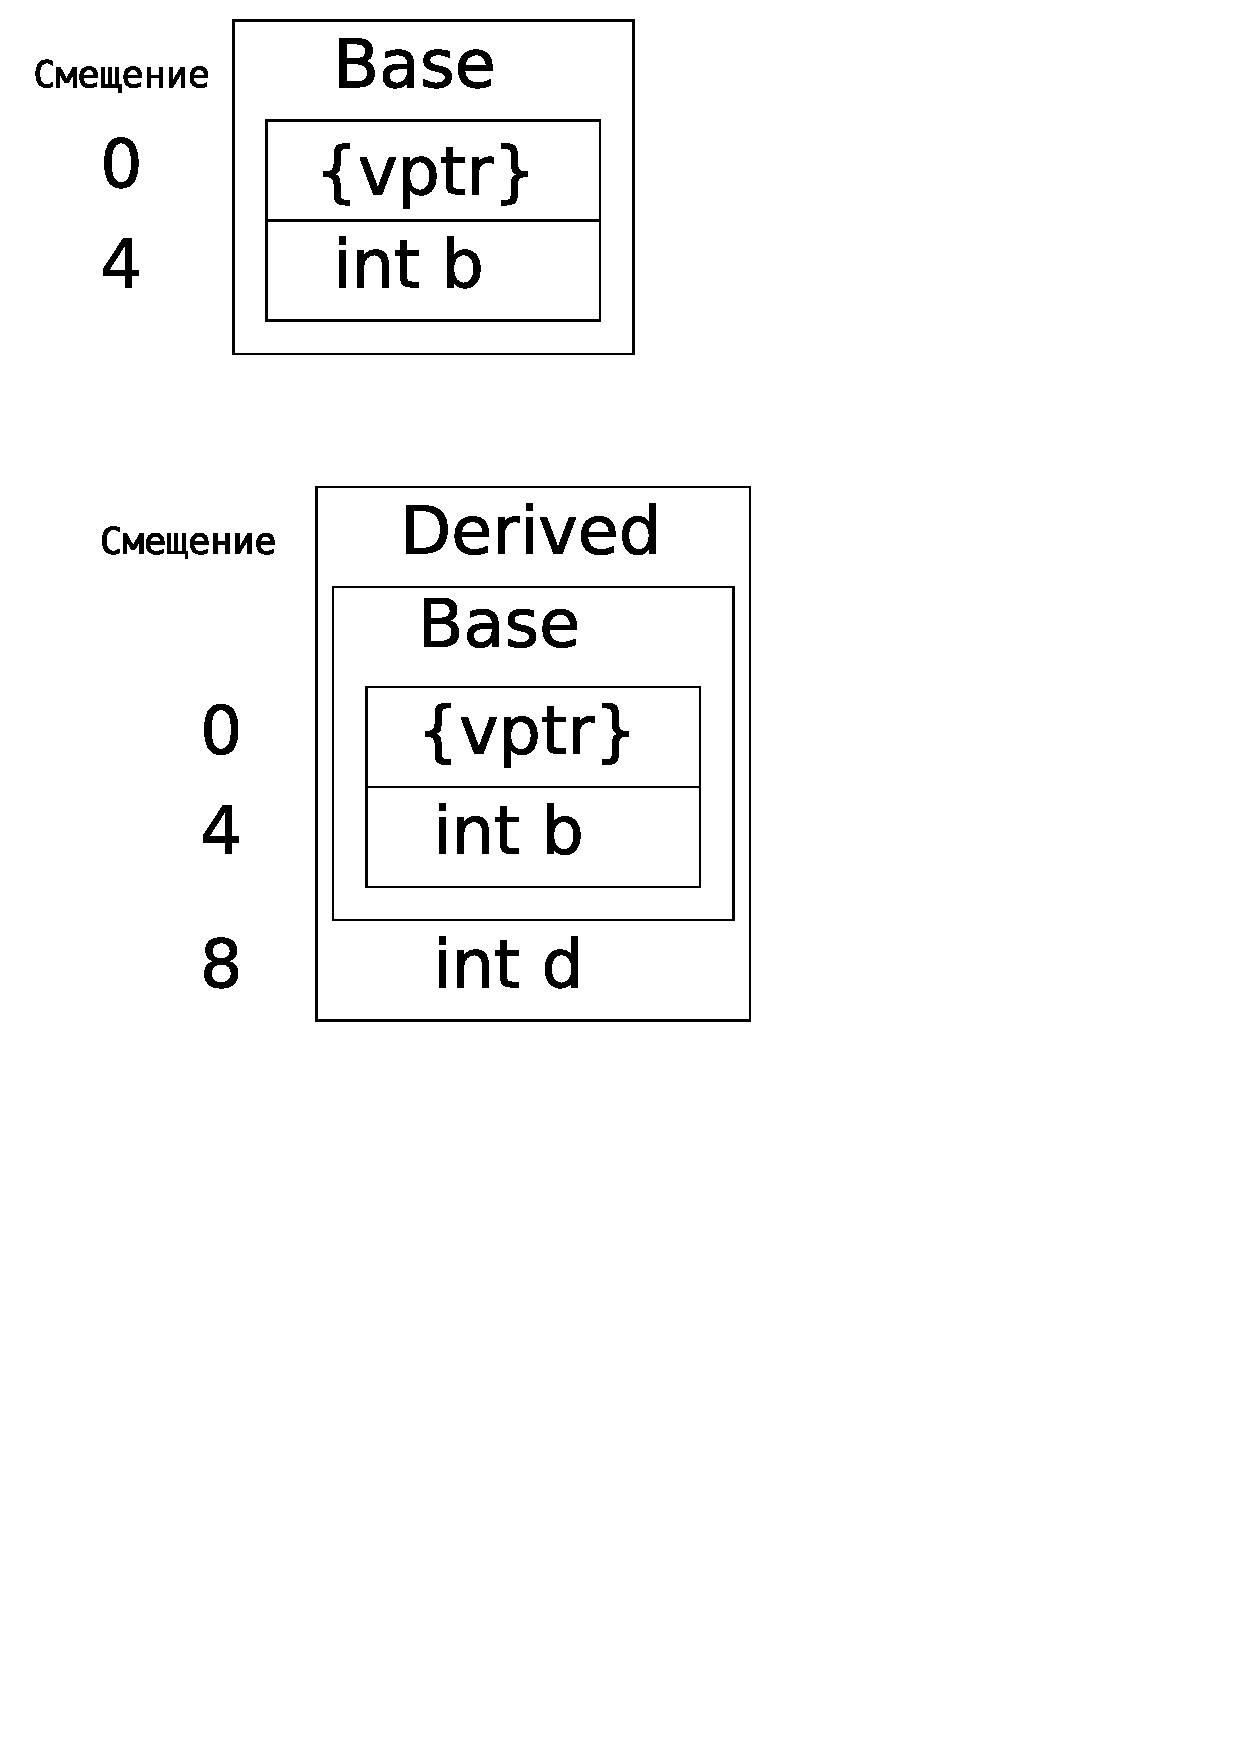
\includegraphics[width=4cm]{simple_mem_layout.pdf}
  \hfill
  \caption{Расположение классов в памяти}
  \label{memlayout_fig}
\end{figure}

Сами таблицы виртуальных функций будут иметь вид, показанный на \picref{simple_vtables_fig}
\begin{figure}
  \center
  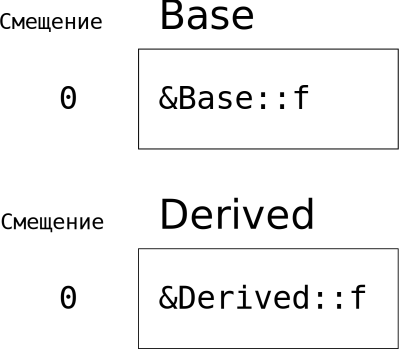
\includegraphics[width=4cm]{simple_vtables.pdf}
  \hfill
  \caption{Расположение в памяти таблиц виртуальных функций}
  \label{simple_vtables_fig}
\end{figure}

Вызов виртуальной функции \texttt{f} происходит следующим образом: по указателю на \texttt{base} находится указатель на таблицу виртуальных функций, из таблицы берется адрес требуемой функции, происходит вызов функции.
\begin{lstlisting}
void test(Base *base) {
  base->f();
}
\end{lstlisting}

\subsection{Метод решения задачи}
Метод решения основывается на анализе таблиц виртуальных функций, а также динамическом анализе потока данных и потока управления.
Принадлежность класса к одной из иерархий можно установить по его указателю на таблицу виртуальных функций.
Однако, равенство указателей на таблицы виртуальных функций не будет означает однозначную принадлежность объектов к одному классу.
Возможна ситуация, когда класс-наследник не переопределяет никаких виртуальных функций.
В этом случае, таблицы виртуальных функций у классов будут одинаковыми.

Принадлежность классов к одной иерархии можно установить, анализируя виртуальные вызовы в программе.
Легко видеть, что все объекты, виртуальные методы которых вызывались одной и той же инструкцией должны принадлежать к одной иерархии классов, и этот вызов происходит через указатель на один из базовых классов. Сравнивая размеры предполагаемые размеры таблиц виртуальных функций можно установить порядок наследования классов.
Анализируя места вызова методов классов можно установить какие из них являются закрытыми (\texttt{private}), т.к. такие методы будут вызываться только из методов соответствующего класса.

\newpage
\section{Инструментальные средства для решения задачи}
\label{valgrind_section}
Для реализации данного инструментального средства требовалась среда, позволяющая проводить динамический анализ программ без наличия исходных кодов.
Предоставление возможности для встраивания функций-перехватчиков и подмены функций семейства \texttt{malloc-free} для анализируемой программы на специальные функции инструментального средства.
Всем этим требованиям отвечает среда Valgrind.

Valgrind представляет собой среду для динамического анализа программ, использующую динамическую рекомпиляцию.
Инструментальное средство, реализованное в с помощью Valgrind'а можно запустить, добавив \texttt{valgrind -{}-tool=<toolname>} перед именем анализируемой программы. Указанное средство запускается, загружает анализируемую программу в адресное пространство своего процесса, и затем рекомпилирует машинный код анализируемой программы небольшими блоками прямо во время исполнения, по мере необходимости.
Ядро дизассемблирует блок кода во внутреннее представление (ВП), которое инструментируется и затем переводится обратно в машинный код.
Никакая часть исходного машинного кода анализируемой программы не запускается в исходном виде. Обрабатываемый корректно код включает в себя обычный исполняемый код, динамически скомпилированные библиотеки, динамически сгенерированный код. Единственный код, который не находится под контролем инструмента --- это системные вызовы, но в Valgrind существует функциональность для получения их побочные эффектов. Множество осложнений возникает при помещении двух программ, анализируемой программы и инструментального средства, в одно адресное пространство. Им приходится 2разделять многие ресурсы, такие как регистры и память.

Цель процесса запуска в том, чтобы поместить ядро Valgrind, инструментальное средство и анализируемую программу в один процесс и одно адресное пространство. Каждое инструментальное средство предоставляет собой статически скомпилированный исполняемый файл, содержащий код ядра и инструментального средства. Исполняемый файл настраивается на загрузку по нестандартному адресу, который, как правило, является свободным при запуске программы (на Linux это \texttt{0x38000000}). Ядро Valgrind сначала инициализирует некоторые подсистемы, такие как управление адресным пространством и свой распределитель памяти. Затем загружается анализируемая программа (секции \texttt{text} и \texttt{data}). Затем настраивается сегмент данных и стек анализируемой программы. Далее ядро вызывает функцию инициализации инструментального средства. В конце инициализируются остальные подсистемы: планировщик потоков, обработчик сигналов и т.д. К этому моменту инструментальное средство и анализируемая программа полностью готовы к работе.

Valgrind транслирует блоки кода при необходимости. Для трансляции блока Valgrind выбирает инструкции, пока не выполнится одно из следующих условий: достигнут предел числа инструкций (около 50, в зависимости от архитектуры), встречен условный переход, встречено ветвление с неизвестным назначением, обработано более 3 безусловных переходов по известным адресам. Существует 8 фаз трансляции. Такое большое число --- следствие подхода, используемого Valgrind. Все фазы берет на себя ядро, за исключением инструментации, выполняемой инструментальным средством. Фазы отмеченные `*' являются архитектурно-зависимыми.

\paragraph{Фаза 1. Дизассемблирование*: машинный код $\to$ дерево ВП.}
Дизассемблер переводит машинный код в не оптимизированное дерево ВП. Каждая инструкция дизассемблируется независимо в один или более операторов.

\paragraph{Фаза 2. Оптимизация 1: дерево ВП $\to$ плоское ВП.}
Первая фаза оптимизации делает ВП плоским и делает некоторые оптимизации: продвижение копий и констант, свёртывание констант, удаление мёртвого кода, удаление общих подвыражений, и даже разворачивание простых циклов.

\paragraph{Фаза 3. Инструментация: плоское ВП $\to$ броское ВП.}
Блок кода передаётся инструментальному средству, которое изменяет его в соответствии со своими требованиями. Важно, чтобы ВП было плоским к этому моменту, это делает инструментацию более простой.

\paragraph{Фаза 4. Оптимизация 2: плоское ВП $\to$ плоское ВП.}
Второй, более простой проход оптимизации выполняет свёртывание констант и удаление мёртвого кода. Эта оптимизация делает жизнь проще для инструментального средства, давая гарантию, что код в последствие будет улучшен.

\paragraph{Фаза 5. Построение дерева: плоское ВП $\to$ дерево ВП.}
Построитель дерева переводит плоское ВП обратно в дерево ВП, готовясь к выбору инструкций. Выражения, присвоенные временным переменным, используемым только один раз перемещаются в точку использования этой временной переменной, а присваивание удаляется. Получаемый код может производить чтения из памяти в другом порядке, но запись в память всегда будет идти после чтения.

\paragraph{Фаза 6. Выбор инструкций*: дерево ВП $\to$ список инструкций.}
В этой фазе дерево ВП переводится в список инструкций, использующих виртуальные регистры (за исключением тех, которые жёстко привязаны к определённым регистрам). Используется просто жадный алгоритм сопоставления образцов, действующий сверху вниз.

\paragraph{Фаза 7. Распределение регистров: список инструкций $\to$ список инструкций.}
Распределитель регистров, использующий линейное сканирование заменяет виртуальные регистры на машинные регистры, вставляя код для сохранения и загрузки значений регистров в память.
Хотя инструкции и зависят от платформы, распределитель регистров является платформенно-независимым.
Он использует функции обратного вызова для получения списков регистров читаемых и записываемых данной инструкцией.

\paragraph{Фаза 8. Ассемблер*: список инструкций $\to$ машинный код.}
Последняя фаза ассемблирования просто кодирует выбранные инструкции и записывает их обратно в блок памяти.

\subsection{Поддержка C++}
Сама среда Valgrind реализована на языке C. Инструменты, реализованные с помощью этой среды также должны быть реализованы на этом языке.
Существует также реализация поддержки для разработки инструментов на C++ (\cite{cppvg}).
Размещение в одном адресном пространстве с анализируемой программой накладывает важное ограничение: ни ядро Valgrind, ни инструмент не могут использовать стандартные библиотеки.
Причина для введения этого ограничения заключается в том, что может возникнуть ситуация, когда одна и та же функция будет исполняться анализируемой программой и самим Valgrind'ом.
Поэтому для использования \texttt{STL}, требуемые части реализации статически связываются с ядром Valgrind.
Реализация вспомогательных функция механизмов исключений и динамической информации о типах находится в разделяемой библиотеке, поэтому единственной способ избавиться от этой зависимости --- это отказаться от использования этих механизмов.

%\addcontentsline{toc}{section}{Заключение}
\newpage
\section{Текущее состояние работы}
Проведен анализ существующих сред для динамического анализа программ, в качестве среды реализации выбран Valgrind.
Реализован прототип инструментального средства с возможностью динамического определения виртуальных вызовов функций, разработана общая архитектура системы.
Реализация будет опираться динамический анализ потока данных и потока управления, определяя таким образом объекты, входящие в одну иерархию.

%% Надо вывести все рисунки до списка литературы
\clearpage

\newpage
\addcontentsline{toc}{section}{Литература}
\begin{thebibliography}{9}
    \bibitem{tydec} \emph{К.Н. Долгова, А.В. Чернов, Е.О. Деревенец} Методы и алгоритмы восстановления программ на языке ассемблера в программы на языке высокого уровня. \textit{Проблемы информационной безопасности, издательство СПГПУ №1 2009.}

    \bibitem{typereconstruction} \emph{K. Dolgova, A. Chernov} Automatic Type Reconstruction in Disassemled C Programs. \textit{Proccedings of WCRE 2008.}

    \bibitem{valgrind} \emph{Nicholas Nethercote, Julian Seward} Proceedings of ACM SIGPLAN 2007 Conference on Programming Language Design and Implementation (PLDI 2007), San Diego, California, USA, June 2007.

    \bibitem{cppvg} \texttt{http://code.google.com/p/data-race-test/wiki/cpp\_vg/}
    \bibitem{strstr} Бьерн Страуструп. Язык программирования С++. М.: Бином, 2006. 1100 с.
    \bibitem{reversing_cpp}P. Sabanal, M. Yason. Reversing C++. Black Hat DC. 2007.
    \bibitem{real_decomp} M. Van Emmerik, T. Waddington. Using a decompiler for real-world source recovery. Proceedings of 11th Working Conference on Reverse Engineering, с. 27-36. 2004.
\end{thebibliography}


\end{document}

%rtti
%ооп
%vtable
%this«Что бы ни произошло, делай вид, что именно этого ты и хотел.»
%abi
%отношение ассоциации (uml)
%поток данных
%поток управления
%алиас
%статический анализ
%динамический анализ